% 1977 年广西卷（理科）参考题 2：线段 AB 上 C、D 为三等分点，以 CD 为直径作园，P 为园周上一点，
% PE 垂直 AB 于 E，θ 为 PC 与 CD 的夹角（按源卷第 5 页布局）
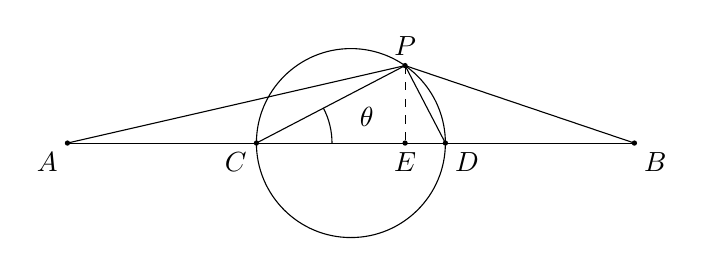
\begin{tikzpicture}[scale=0.8]
  \coordinate (A) at (0,0);
  \coordinate (C) at (3,0);
  \coordinate (D) at (6,0);
  \coordinate (B) at (9,0);
  \coordinate (P) at (5.36,1.23);
  \coordinate (E) at (5.36,0);
  \draw (A)--(B);
  \draw (4.5,0) circle (1.5);
  \draw (A)--(P);
  \draw (B)--(P);
  \draw (P)--(C);
  \draw (P)--(D);
  \draw[dashed] (P)--(E);
  \draw (4.2,0) arc(0:27.5:1.2);
  \node at (4.75,0.42) {$\theta$};
  \fill (A) circle (1.2pt) node[below left] {$A$};
  \fill (B) circle (1.2pt) node[below right] {$B$};
  \fill (C) circle (1.2pt) node[below left] {$C$};
  \fill (D) circle (1.2pt) node[below right] {$D$};
  \fill (E) circle (1.2pt) node[below] {$E$};
  \fill (P) circle (1.2pt) node[above] {$P$};
\end{tikzpicture}
